\documentclass[11pt]{article} % use larger type; default would be 10pt


%%% PAGE DIMENSIONS
\usepackage[top=1in, bottom=1in, left=0.5in, right=0.5in]{geometry} % to change the page dimensions
 
%%% PACKAGES
\usepackage{graphicx} % support the \includegraphics command and options
\usepackage{amsfonts}
\usepackage{amsmath}
\usepackage{tikz}
\usepackage{graphicx}
\usepackage{color}
\usepackage{bbm}
\usetikzlibrary{arrows}
%%% The "real" document content comes below...

\title{CS 134: Networks \\ \emph{Problem Set 9}}
\author{Xiner Zhou}
\date{\today} % Activate to display a given date or no date (if empty),
        

\begin{document}
 
\maketitle

 \paragraph{1. How to Win the Web  (Easley and Kleinberg, 14.7 Q3) (20 points)}
 
\begin{itemize}
\item[\textbf{a. }] \textcolor{red}{Solution:}

$$\begin{array} {|c | c c c c c c|} \hline
 & \text{A} & \text{B} & \text {C} & \text {D} & \text {E} & \text{F}  \\ \hline
a^{(1)} & 3 & 2 &  0 & 0 & 0 & 0 \\ 
h^{(1)} & 0 & 0 &  3 & 3 & 5 & 2  \\  
a^{(2)} & 11 & 7 &  0 & 0 & 0 & 0  \\  
h^{(21)} & 0 & 0 &  11 & 11 & 18 & 7  \\ \hline
\text{Normaized} \ a^{(2)} & \frac{11}{18} & \frac{7}{18}  &  0 & 0 & 0 & 0 \\  
\text{Normaized} \  h^{(2)}  & 0 & 0 & \frac{11}{47}  & \frac{11}{47} & \frac{18}{47}  & \frac{7}{47} \\ \hline
\end{array}$$

\item[\textbf{b. }]  \textcolor{red}{Solution:}
\textbf{Option 1:}
$$\begin{array} {|c | c c c c c c c c|} \hline
 & \text{A} & \text{B} & \text{X} & \text {C} & \text {D} & \text {E} & \text{F}  & \text{Y}\\ \hline
a^{(1)} & 3 & 2 & 1 &  0 & 0 & 0 & 0 & 0\\ 
h^{(1)} & 0 & 0 &  0 & 3 & 3 & 5 & 2 & 1 \\  
a^{(2)} & 11 & 7 & 1 & 0 & 0 & 0 & 0  & 0\\  
h^{(21)} & 0 & 0 & 0 &  11 & 11 & 18 & 7 & 1  \\ \hline
\text{Normaized} \ a^{(2)} & \frac{11}{19}  & \frac{7}{19}    & \frac{1}{19}   &  0 & 0 & 0 & 0 & 0 \\  
\text{Normaized} \  h^{(2)}  & 0 & 0  & 0 & \frac{11}{48}   & \frac{11}{48}  & \frac{18}{48} & \frac{7}{48}   & \frac{1}{48}  \\ \hline
\end{array}$$

\textbf{Option 2:}
$$\begin{array} {|c | c c c c c c c c|} \hline
 & \text{A} & \text{B} & \text{X} & \text {C} & \text {D} & \text {E} & \text{F}  & \text{Y}\\ \hline
a^{(1)} & 4 & 3 & 1 &  0 & 0 & 0 & 0 & 0\\ 
h^{(1)} & 0 & 0 &  0 & 4 & 4 & 7 & 3 & 8 \\  
a^{(2)} & 18 & 18 & 8 & 0 & 0 & 0 & 0  & 0\\  
h^{(21)} & 0 & 0 & 0 &  18 & 18 & 36 & 18 & 44  \\ \hline
\text{Normaized} \ a^{(2)} & \frac{18}{44}  & \frac{18}{44}    & \frac{8}{44}   &  0 & 0 & 0 & 0 & 0 \\  
\text{Normaized} \  h^{(2)}  & 0 & 0  & 0 & \frac{18}{134}   & \frac{18}{134}  & \frac{36}{134}&\frac{18}{134} & \frac{44}{134}  \\ \hline
\end{array}$$

Option 2 gives higher authority score for X. Intuitively, in the HITS algorithm, page X's authority score is proportional to the sum of hub scores of the pages that point to it, in this case, only Y. and Y's hub score is proportional to the sum of the authority scores of the pages it points to. In option 2, Y gets the highest hub score by pointing to both A and B, while in option 1, Y gets the lowest hub score, compared to C,D,E, and F. Therefore, in option 2, Y's vote is more important than that in option 1. The page benefits the most is the page X, its relative rank of authority score goes up.

\item[\textbf{c. }] \textcolor{red}{Solution:} 
Add new nodes X, Y, and Z, create links from Y to A and X, and create links from Z to A and X.

\begin{center}
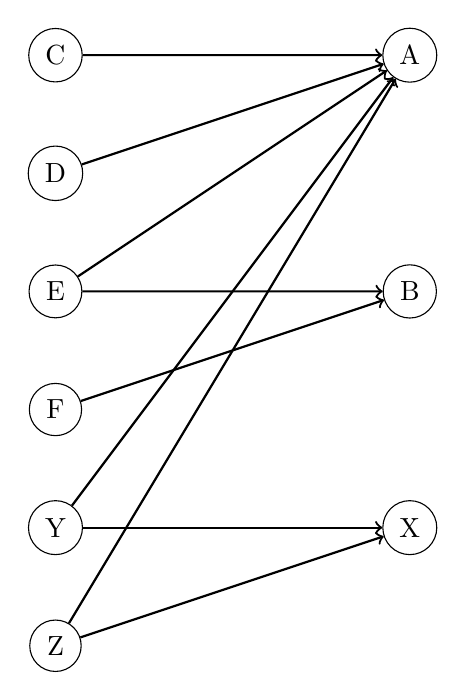
\begin{tikzpicture}[node distance=2cm, scale=1.5]

\node[draw, shape=circle ] (Z) at (0,0 ) {Z};
\node[draw, shape=circle ] (Y)  at (0,1) {Y};
\node[draw, shape=circle ] (F)  at (0, 2) {F};
\node[draw, shape=circle ] (E)  at (0, 3){E};
 \node[draw, shape=circle ] (D)  at (0, 4){D};
\node[draw, shape=circle ] (C)  at (0, 5){C};

\node[draw, shape=circle ] (X)  at (3, 1){X};
\node[draw, shape=circle ] (B)  at (3, 3){B};
\node[draw, shape=circle ] (A)  at (3, 5){A};

\draw[->, thick] (C) to (A);
\draw[->, thick] (D) to (A);
\draw[->, thick] (E) to (A);
\draw[->, thick] (E) to (B);
\draw[->, thick] (F) to (B);
\draw[->, thick] (Y) to (A);
\draw[->, thick] (Y) to (X);
\draw[->, thick] (Z) to (A);
\draw[->, thick] (Z) to (X);
\end{tikzpicture}
\end{center}

$$\begin{array} {|c | c c c c c c c c c|} \hline
 & \text{A} & \text{B} & \text{X} & \text {C} & \text {D} & \text {E} & \text{F}  & \text{Y}  & \text{Z}\\ \hline
a^{(1)} & 5 & 2 & 2 &  0 & 0 & 0 & 0 & 0 & 0\\ 
h^{(1)} & 0 & 0 &  0 & 5 & 5 & 7 & 2 & 7 & 7\\  
a^{(2)} &  31 & 9 & 14 & 0 & 0 & 0 & 0  & 0 & 0\\  
h^{(21)} & 0 & 0 & 0 &  31 & 31 & 40 & 9 & 45& 45  \\ \hline
\text{Normaized} \ a^{(2)} & \frac{31}{54}  & \frac{9}{54}    & \frac{14}{54}   &  0 & 0 & 0 & 0 & 0 & 0 \\  
\text{Normaized} \  h^{(2)}  & 0 & 0  & 0 & \frac{31}{201}   & \frac{31}{201}     & \frac{40}{201}   & \frac{9}{201}    & \frac{45}{201} & \frac{45}{201}    \\ \hline
\end{array}$$

Rank by authority score: $A > X > B > C,D,E,F,Y,Z$.
\end{itemize}













\paragraph{2. Limiting Values of PageRank  (Easley and Kleinberg, 14.7 Q4) (20 points)}
 
\begin{itemize}
\item[\textbf{a. }]  \textcolor{red}{Solution:}

$$r^{(t)}=\left( \begin{array}{c}
3/10 \\
1/10 \\
2/10 \\
1/10 \\
3/10
\end{array}\right) $$

The transition matrix:
$$ M=\left( \begin{array}{ccccc}
0 & 1/3 & 1/3 & 1/3 & 0\\
0 & 0 &1/2 & 0 & 1/2 \\
0 & 0 &0 & 0 & 1\\
0 & 0 &1/2 & 0 & 1/2\\
1 & 0 &0 & 0 & 0
\end{array}\right) $$


$$\Rightarrow \sum_{j \in {A,B,C,D,E}} r_j^{(t)}=1$$
and
$$r^{(t+1)}=M^T r^{(t)}= \left( \begin{array}{c}
3/10 \\
1/10 \\
2/10 \\
1/10 \\
3/10
\end{array}\right) = r^{(t)}$$
PageRank values remain unchanged when we apply the Basic PageRank Update Rule. Therefore, the assignment of numbers to the nodes form an equilibrium set of PageRank values.


\item[\textbf{b. }]  \textcolor{red}{Solution:}
$$r^{(t)}=\left( \begin{array}{c}
1/4\\
1/8\\
1/8\\
1/8\\
1/4\\
1/8
\end{array}\right) $$

The transition matrix:
$$ M=\left( \begin{array}{cccccc}
0 & 1/2 & 1/2 & 0 & 0 & 0\\
0 & 0 & 0 &1/2 & 1/2 & 0\\
0 & 0 &0 & 0 &1/2 & 1/2\\
1 & 0 & 0 & 0 & 0 & 0\\
1 & 0 & 0 & 0 & 0 & 0\\
1 & 0 & 0 & 0 & 0 & 0
\end{array}\right) $$


$$\Rightarrow \sum_{j \in {A,B,C,D,E,G}} r_j^{(t)}=1$$
and
$$r^{(t+1)}=M^T r^{(t)}= \left( \begin{array}{c}
1/2\\
1/8\\
1/8\\
1/16\\
1/8\\
1/16
\end{array}\right) \neq r^{(t)}$$
PageRank values changes when we apply the Basic PageRank Update Rule. Therefore, the assignment of numbers to the nodes does \textcolor{red}{NOT} form an equilibrium set of PageRank values.

\end{itemize}
 





















\paragraph{3. Avoiding Undesirable Equilibria in PageRank (20 points)}
 
\begin{itemize}
\item[\textbf{a. }] \textcolor{red}{Solution:}
The transition matrix:
$$ M=\left( \begin{array}{cccccccc}
0 & 1/2 & 1/2 & 0 & 0 & 0 & 0 & 0\\
0 & 0 & 0 &1/2 & 1/2 & 0 & 0 & 0\\
0 & 0 &0 & 0 & 0 &1/2 & 1/2 & 0\\
1/2 & 0 & 0 & 0 & 0 & 0 & 0 &1/2\\
1/2 & 0 & 0 & 0 & 0 & 0 & 0 &1/2\\
0 & 0 & 0 & 0 & 0 & 0 & 1 & 0\\
0 & 0 & 0 & 0 & 0 & 1 & 0 & 0\\
1 & 0 & 0 & 0 & 0 & 0 & 0 & 0
\end{array}\right) $$

If the equilibrium set of PageRank values exists, i.e., $$ \lim_{t \to \infty} r^{(t)}=  r^{*}$$ 
then it should remain unchanged when we apply the Basic PageRank Update Rule, i.e., $$M^T r^{*}=r^{*}$$

Therefore, $r^{*}$ is the eigenvector of $M^T$ corresponding to the eigenvalue 1 (calculation using Python). 

$$ \Rightarrow  \lim_{t \to \infty} r^{(t)}=  r^{*}= \left( \begin{array}{c}
0\\
0\\
0\\
0\\
0\\
0.5\\
0.5\\
0
\end{array}\right) $$

\item[\textbf{b. }] \textcolor{red}{Solution:}
All PageRank equilibria in $G$ give non-zero PageRank valeus to all nodes, if and only iff, the directed graph $G$ is strongly connected ($G$ is itself one big strongly connected component SCC).

\textbf{Proof:} \\
$\Rightarrow :$ Since the PageRank value of a node $v$ is exactly the probability of a random walk that starts from any random node $u \in V$ and lands on $v$, if all PageRank equilibria in $G$ give non-zero PageRank valeus to all nodes, then a random walk starting from any node $u \in V$ can land on any node $ v \in V$ with positive probability, that means, there is a path from every node to every other node, i.e., $G$ is strongly connected.

$\Leftarrow :$ If $G$ is strongly connected, i.e., there is a path from every node to every other node, therefore, the probability of a random walk that starts from any random node $u \in V$ and lands on any node $ v \in V$ is positive, it is equivalent to say that, the PageRank equilibria of any node $ v >0$.

\end{itemize}
 


















\paragraph{4. Detecting Link Farms (Easley and Kleinberg, 14.7 Q6) (20 points)}
 
\begin{itemize}
\item[\textbf{a. }]\textcolor{red}{Solution:}

$$\begin{array} {|c | c c c c c c c c c c c c|} \hline
 & \text{$A_1$} & \text{$A_2$} & \text{$A_3$} & \text{$B_1$} & \text{$B_2$} & \text{$B_3$} & \text{$C_1$}  & \text{$C_2$}  & \text{$C_3$} & \text{$C_4$} & \text{$C_5$} & \text{$D$}\\ \hline
a^{(1)} & 0 & 0 & 0 &  3 & 3 & 3 & 0 & 0 & 0 & 0 & 0 & 5\\ 
h^{(1)} & 9 & 9 &  9 & 0 & 0 & 0 & 5 & 5 & 5 & 5 & 5 & 0\\  
a^{(2)} & 0 & 0 & 0 & 27 & 27 & 27 & 0  & 0 & 0 & 0  & 0 & 25\\  
h^{(2)} & 81 & 81 & 81 &  0 & 0 & 0 & 25 & 25& 25  & 25& 25 & 0\\ \hline
\text{Normaized} \ a^{(2)} & 0 & 0 & 0 & \frac{27}{106} & \frac{27}{106} & \frac{27}{106} & 0  & 0 & 0 & 0  & 0 & \frac{25}{106}\\  
\text{Normaized} \  h^{(2)}  & \frac{81}{368} & \frac{81}{368} & \frac{81}{368} &  0 & 0 & 0 & \frac{25}{368} & \frac{25}{368}&\frac{25}{368}  & \frac{25}{368}& \frac{25}{368} & 0\\ \hline
\end{array}$$



\item[\textbf{b. }]\textcolor{red}{Solution:} 

$$\begin{array} {|c | c c c c c c |} \hline
 & \text{$A_1$} & \text{$A_2$} & \text{$A_3$} & \text{$B_1$} & \text{$B_2$} & \text{$B_3$} \\ \hline 
a^{(k)} & 0 & 0 & 0 & 3^{2k-1} & 3^{2k-1} & 3^{2k-1}  \\  
h^{(k)} & 3^{2k}& 3^{2k} & 3^{2k}&  0 & 0 & 0  \\ \hline
\text{Normaized} \ a^{(k)} & 0 & 0 & 0 & \frac{3^{2k-1}}{3^{2k}+5^k} & \frac{3^{2k-1}}{3^{2k}+5^k}  & \frac{3^{2k-1}}{3^{2k}+5^k}   \\  
\text{Normaized} \  h^{(k)}  & \frac{3^{2k}}{3^{2k}+5^{k+1}} & \frac{3^{2k}}{3^{2k}+5^{k+1}} & \frac{3^{2k}}{3^{2k}+5^{k+1}} &  0 & 0 & 0  \\ \hline
\end{array}$$

$$\begin{array} {|c | c c c c c c |} \hline
 &  \text{$C_1$}  & \text{$C_2$}  & \text{$C_3$} & \text{$C_4$} & \text{$C_5$} & \text{$D$}\\ \hline 
a^{(k)}  & 0  & 0 & 0 & 0  & 0 & 5^k\\  
h^{(k)}  & 5^k & 5^k& 5^k  & 5^k& 5^k & 0\\ \hline
\text{Normaized} \ a^{(k)}  & 0  & 0 & 0 & 0  & 0 & \frac{5^k}{3^{2k}+5^k} \\  
\text{Normaized} \  h^{(k)}   & \frac{5^k}{3^{2k}+5^{k+1}} & \frac{5^k}{3^{2k}+5^{k+1}} & \frac{5^k}{3^{2k}+5^{k+1}}  & \frac{5^k}{3^{2k}+5^{k+1}} & \frac{5^k}{3^{2k}+5^{k+1}} & 0\\ \hline
\end{array}$$


\item[\textbf{c. }] \textcolor{red}{Solution:} 
Since $$ \lim_{k \to \infty} \frac{3^{2k-1}}{3^{2k}+5^k}=\frac{1}{3}$$
$$ \lim_{k \to \infty} \frac{5^k}{3^{2k}+5^k}=0$$ 
$$ \lim_{k \to \infty} \frac{3^{2k}}{3^{2k+1}+5^{k+1}}=\frac{1}{3}$$
$$ \lim_{k \to \infty} \frac{5^k}{3^{2k}+5^{k+1}}=0$$ 
Therefore, as $k$ goes infinity, the authority score of $B_1$, $B_2$, and $B_3$ goes to $\frac{1}{3}$, while the authority score of $D$ goes to 0 (other pages always have authority score of 0). And the hub score of $A_1$, $A_2$, and $A_3$ goes to $\frac{1}{3}$ ,while the authority score of  $C_1$, $C_2$, $C_3$, $C_4$, and $C_5$, goes to 0 (other pages always have authority score of 0). 

\textbf{Computationally:} Before final normalization, the authority score of $B_1$, $B_2$, and $B_3$ grow exponentially by a factor of $3^2=9$ each iteration, while $D$ only grows exponentially by a factor of $5^1=5$ during each iteraction, therefore, as $t$ goes to infinity, $B_1$, $B_2$, and $B_3$ equally dominate the share of the total authority score, while $D's$ relative authority score goes smaller and smaller to 0. The same reasoning applied to the hub scores.

\textbf{Intuitively:} In terms of the authority scores, pages that have multiple reinforcing endorsements, in this case, $B_1$, $B_2$, and $B_3$, their "reference" pages' hub scores  (that endorse them) also grow by a factor equals to number of reference pages, by the mechanism of multiple reinforcing endorsement; for pages (in tjhis case $D$) that simply have high in-degree, the "reference" pages' hub scores stay the same in each iteraction as $D's$ authority score, which leads to a lower grow rate of $D's$ authority score in the long run, compared to pages that have multiple reinforcing endorsements. Therefore, in relative term, or after normalization, $D's$ authority score goes to oblivous, while $B_1$, $B_2$, and $B_3$ dominate the prominent positions.

\end{itemize}

















\paragraph{5. Implementing PageRank (20 points)}
 
\begin{itemize}
    \item[\textbf{b. }]\textcolor{red}{Solution:}  
 There are 387,597 nodes, and the average out-degree is 1.37. Because of time constraint, I wasn't able to implement the algorithm for the entire network, therefore, I used a ranom sample of size 10,000, for Q5 c- Q5e. The algorithm run without error, I suppose if given more time, they will generate accurate full picture of the whole network. Please check my codes at "pset9 Code Xiner Zhou.py" for details.

    \item[\textbf{c. }]\textcolor{red}{Solution:}  
\begin{center}
\includegraphics[width=8in, height=4in]{Q5c.png}
\end{center}
Based on the histogram, power law distribution or the rich-get-richer model might be a good candicate for these google pages
    \item[\textbf{d. }]\textcolor{red}{Solution:} 
\begin{center}
\textbf{k=10:}
\includegraphics[width=8in, height=4in]{Q5dk10.png}
\textbf{k=50:}
\includegraphics[width=8in, height=4in]{Q5dk50.png}
\textbf{k=200:}
\includegraphics[width=8in, height=4in]{Q5dk200.png}
\end{center}
    \item[\textbf{e. }]\textcolor{red}{Solution:} 
\begin{center}
\textbf{k=10:}
\includegraphics[width=8in, height=4in]{Q5ek10.png}
\textbf{k=50:}
\includegraphics[width=8in, height=4in]{Q5ek50.png}
\textbf{k=200:}
\includegraphics[width=8in, height=4in]{Q5ek200.png}
\end{center}

    \item[\textbf{f. }]\textcolor{red}{Solution:}  
Not enough time to complete this part.
\end{itemize}
 
 
\end{document}
